\documentclass[letterpaper, 11pt]{article} 

\usepackage{graphics,graphicx}
\usepackage{multicol} 
\usepackage{parskip}
\usepackage{amsmath}
\usepackage{multirow}
\usepackage[utf8]{inputenc}
\usepackage{fancyhdr}
\usepackage[title]{appendix}
\usepackage{wasysym}
\usepackage{url}
\usepackage{subcaption}

\usepackage[font=footnotesize,labelfont=small]{caption}
\captionsetup{width=0.85\linewidth}

\RequirePackage{geometry}
\geometry{margin=2cm}

\setlength{\parskip}{0.2cm}
\setlength{\parindent}{0pt}


\title{Lab Report 5: Design 2-to-1 Mux}
\author{
Tai Duc Nguyen \\
ECEC 471: Introduction to VLSI
}
\date{\today}

\begin{document}

\maketitle


%----------------------------------------------------------------------------------------
%	ABSTRACT
%----------------------------------------------------------------------------------------


\rule{\textwidth}{1pt}

\begin{abstract}
A multiplexer (mux) is a common component used in many circuits. A mux is used when multiple data lines (input $a_1, a_2,...,a_n$) share a single data line (output $q$), and the select bits ($sel$) are used to determine which inputs are chosen to connect to the output. In this laboratory, the schematic and layout design of the 2-to-1 mux (will only be refered as mux in the future) will be determined using Cadence Virtuoso and verified through tools such as DRC and LVS in the Cadence Interactive Toolbox.
\end{abstract}

\rule{\textwidth}{1pt}

\section{Introduction}
\label{sec:intro}

%\begin{multicols}{2}
Multiplexer is a basic component which is mainly used as control gate in complex digital circuits. This lab's mux is comprised of 3 NAND logic gate and 1 inverter (INV) connected together and shown in Figure \ref{fig1a} below. As the number of input lines ($N$) increases, the number of select bits increase ($S=ceil(log_2(n))$). A 4-to-1 multiplexer will look like Figure \ref{fig1b}.

\begin{figure}[ht!]
	\centering
	\begin{subfigure}[b]{.3\linewidth}
		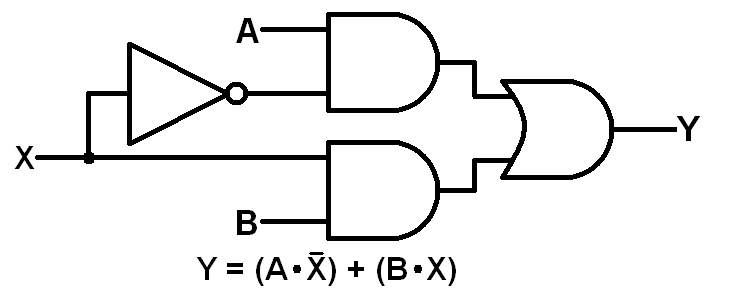
\includegraphics[width=\textwidth]{2_to_1_mux.png}
		\caption{2-to-1 mux}
		\label{fig1a}
	\end{subfigure}
	\hskip2em
	\begin{subfigure}[b]{.3\linewidth}
		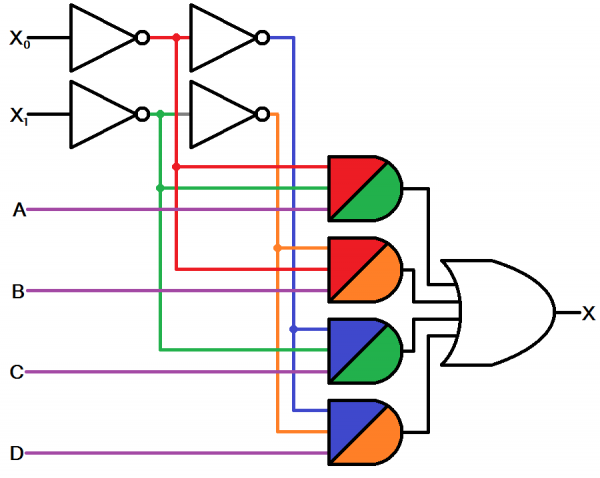
\includegraphics[width=\textwidth]{4_to_1_mux.png}
		\caption{4-to-1 mux}
		\label{fig1b}
	\end{subfigure}
	\caption{Logic gate layout of multiplexers (https://learn.sparkfun.com/tutorials/logicblocks-experiment-guide/7-2-to-1-multiplexer)}
\end{figure}


\section{Schematic Design}
\label{sec:schematic_design}
The following Figure \ref{fig2} is the result of the mux layout in Cadence Virtuoso. The connections between the logic gates are similar to that of Figure \ref{fig1a}. The individual NAND gates and inverters are imported from previously symmetrically built components.

\begin{figure}[htb!]
	\centering
	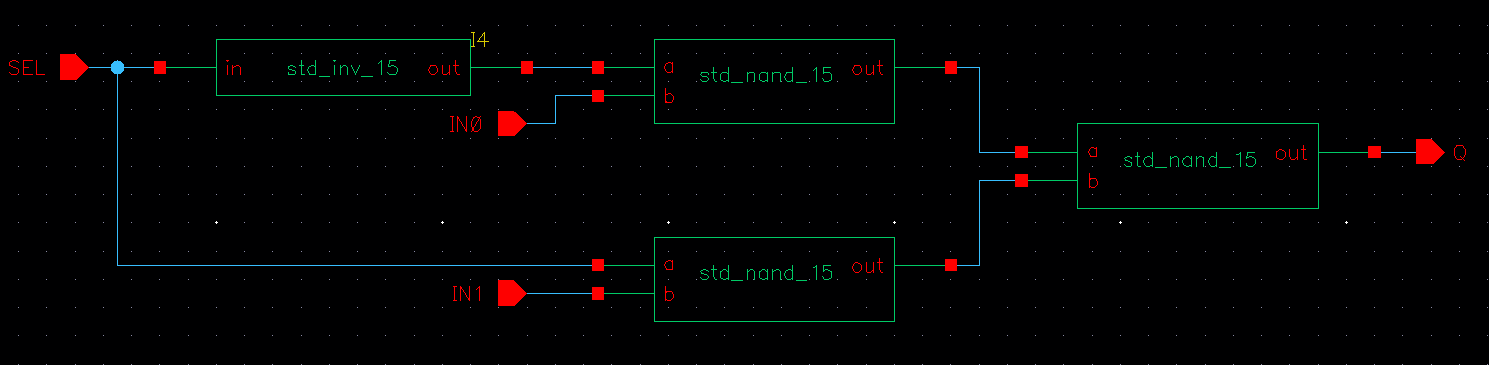
\includegraphics[width=1.0\linewidth]{mux_schematic_final.png}
	\caption{2-to-1 mux's schematic layout}
	\label{fig2}
\end{figure}

After the schematic is laid out, the symbol for the mux is created and the entire inner working of the circuitry is simulated with the layout in Figure \ref{fig3} below.

\begin{figure}[htb!]
	\centering
	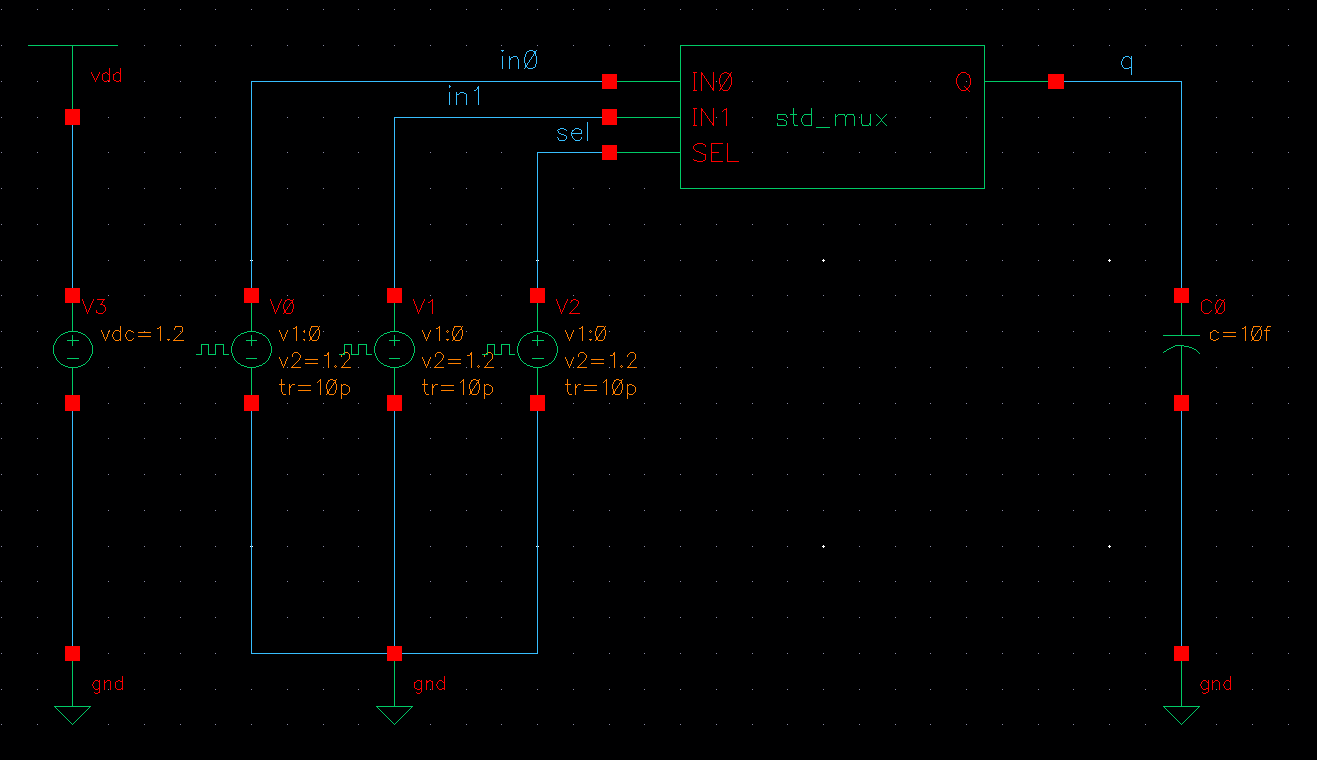
\includegraphics[width=0.9\linewidth]{mux_sim_schematic.png}
	\caption{2-to-1 mux's simulation layout}
	\label{fig3}
\end{figure}

\section{Schematic Simulation and Results}
\label{sec:schematic_sim_and_res}

This section documents the simulation steps and their results. First, table \ref{table1} below shows the combinations of the inputs and their respective output values of the mux
\begin{table}[htb!]
	\centering
	\begin{tabular}{l|l|l|l}
		IN0 & IN1 & SEL & Q \\ \hline
		0 & 1 & 0 & 0 \\
		0 & 1 & 1 & 1 \\
		1 & 0 & 0 & 1 \\
		1 & 0 & 1 & 0
	\end{tabular}
	\caption{2-to-1 mux's table of input to output combinations}
	\label{table1}
\end{table}

From the simulation layout above, the transient analysis of this mux can be performed using ADE(L) simulation tool. The graph of this analysis is shown in Figure \ref{fig4}. Derived from the figure is the information of different delays, rise, and fall time characteristics.

\begin{figure}[htb!]
	\centering
	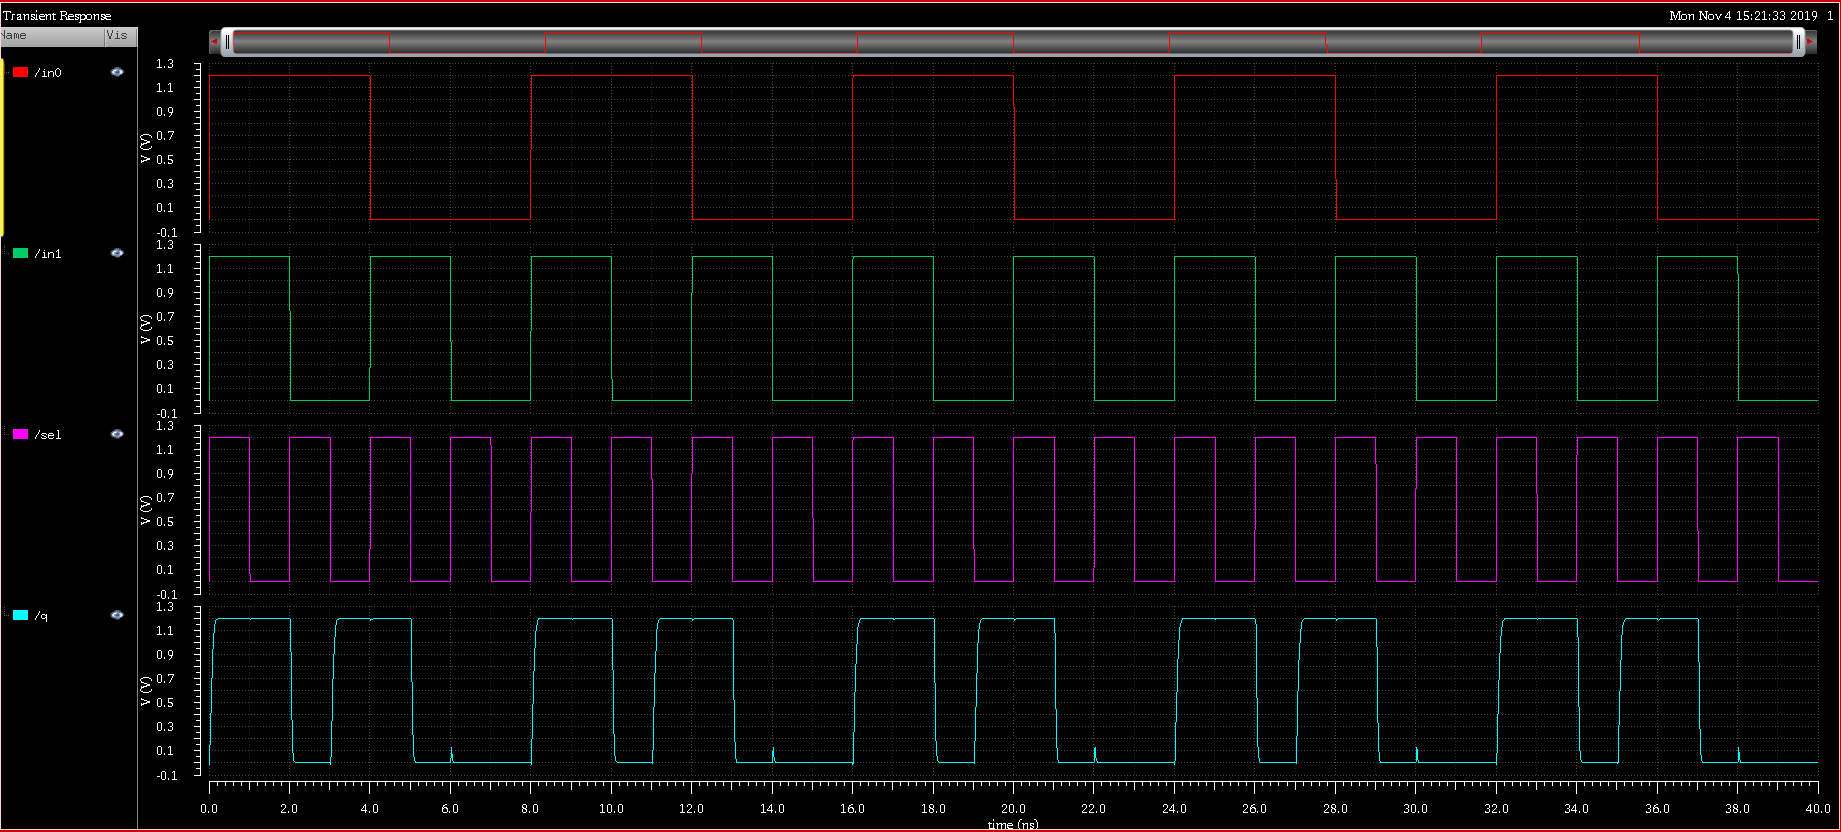
\includegraphics[width=0.8\linewidth]{mux_transient_init.png}
	\caption{2-to-1 mux's ADE(L) simulated transient plot}
	\label{fig4}
\end{figure}


Since there are 4 cases - 4 different combinations of inputs, the delays for each case are calculated and documents in table \ref{table2}. 

\begin{table}[htb!]
	\centering
	\begin{tabular}{l|l|l|l|l}
		IN0 & IN1 & SEL & Q & Delay\\ \hline
		0 & 1 & 0 & 0 & 0.03421 \\
		0 & 1 & 1 & 1 & 0.06057 \\
		1 & 0 & 0 & 1 & 0.05170 \\
		1 & 0 & 1 & 0 & 0.04496
	\end{tabular}
	\caption{2-to-1 mux's table of input to output combinations with their respective delays}
	\label{table2}
\end{table}

These calculations result from generating 2 configurations of the simulation schematic. In the first configuration, the IN1 has a delay of 0ns, and in the second configuration, the IN1 has a delay of 2ns (Figure \ref{fig5a} \& \ref{fig5b}).

\begin{figure}[htb!]
	\centering
	\begin{subfigure}[htb]{.9\linewidth}
		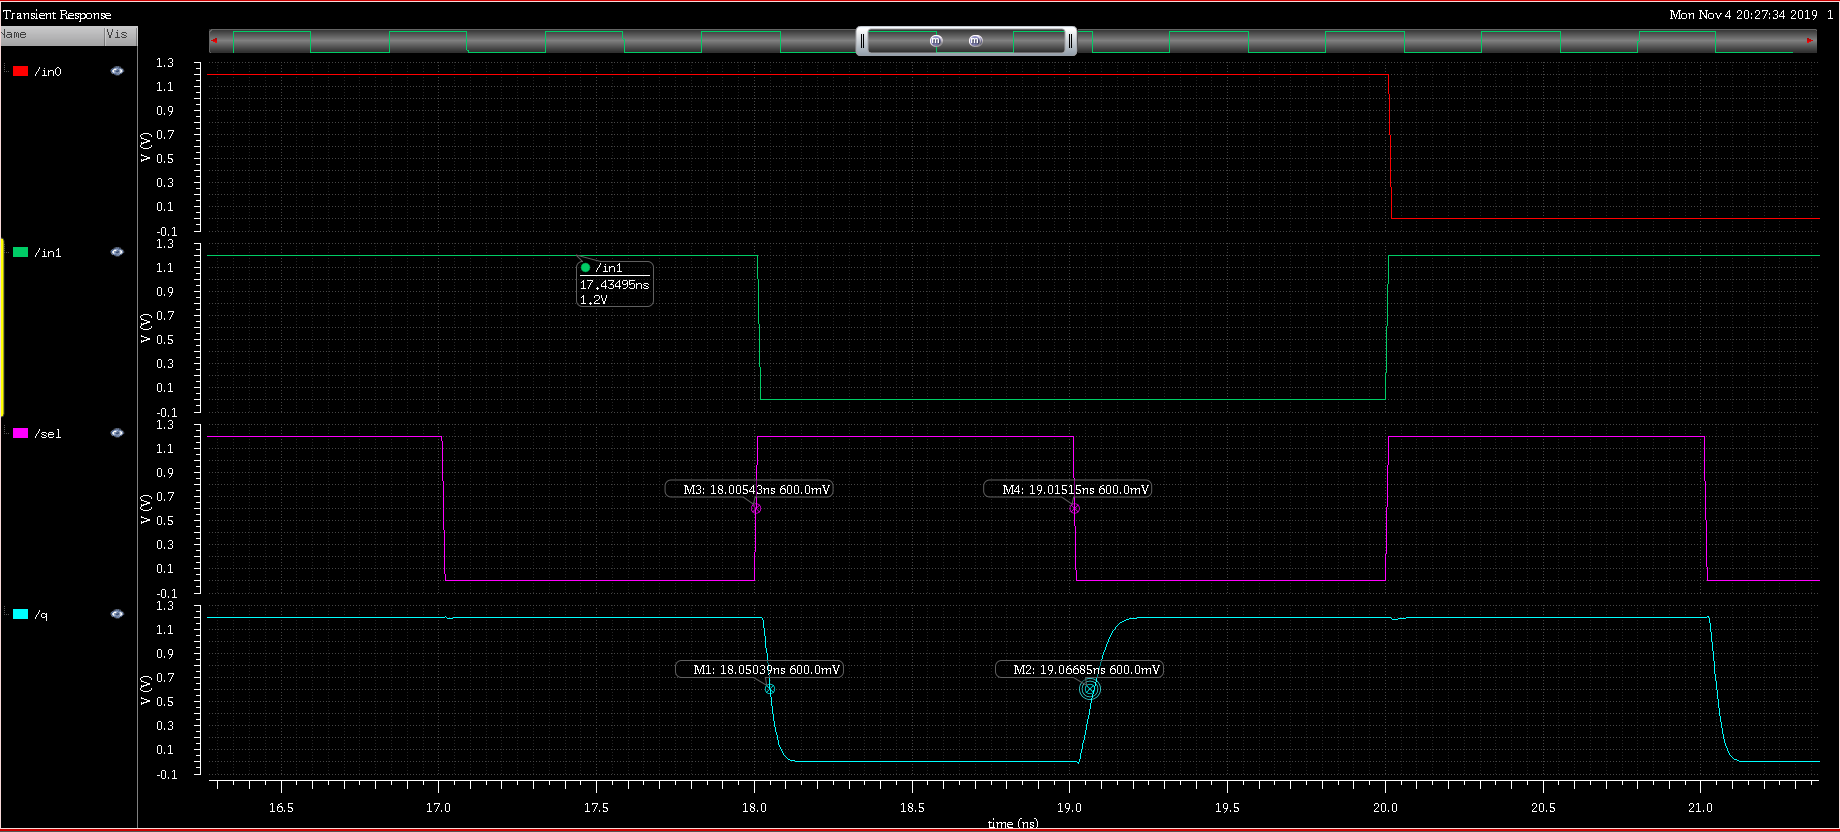
\includegraphics[width=\textwidth]{mux_prop_delay_1.png}
		\caption{First configuration's propagation delays}
		\label{fig5a}
	\end{subfigure}
	%	\hskip2em
	\begin{subfigure}[htb]{.9\linewidth}
		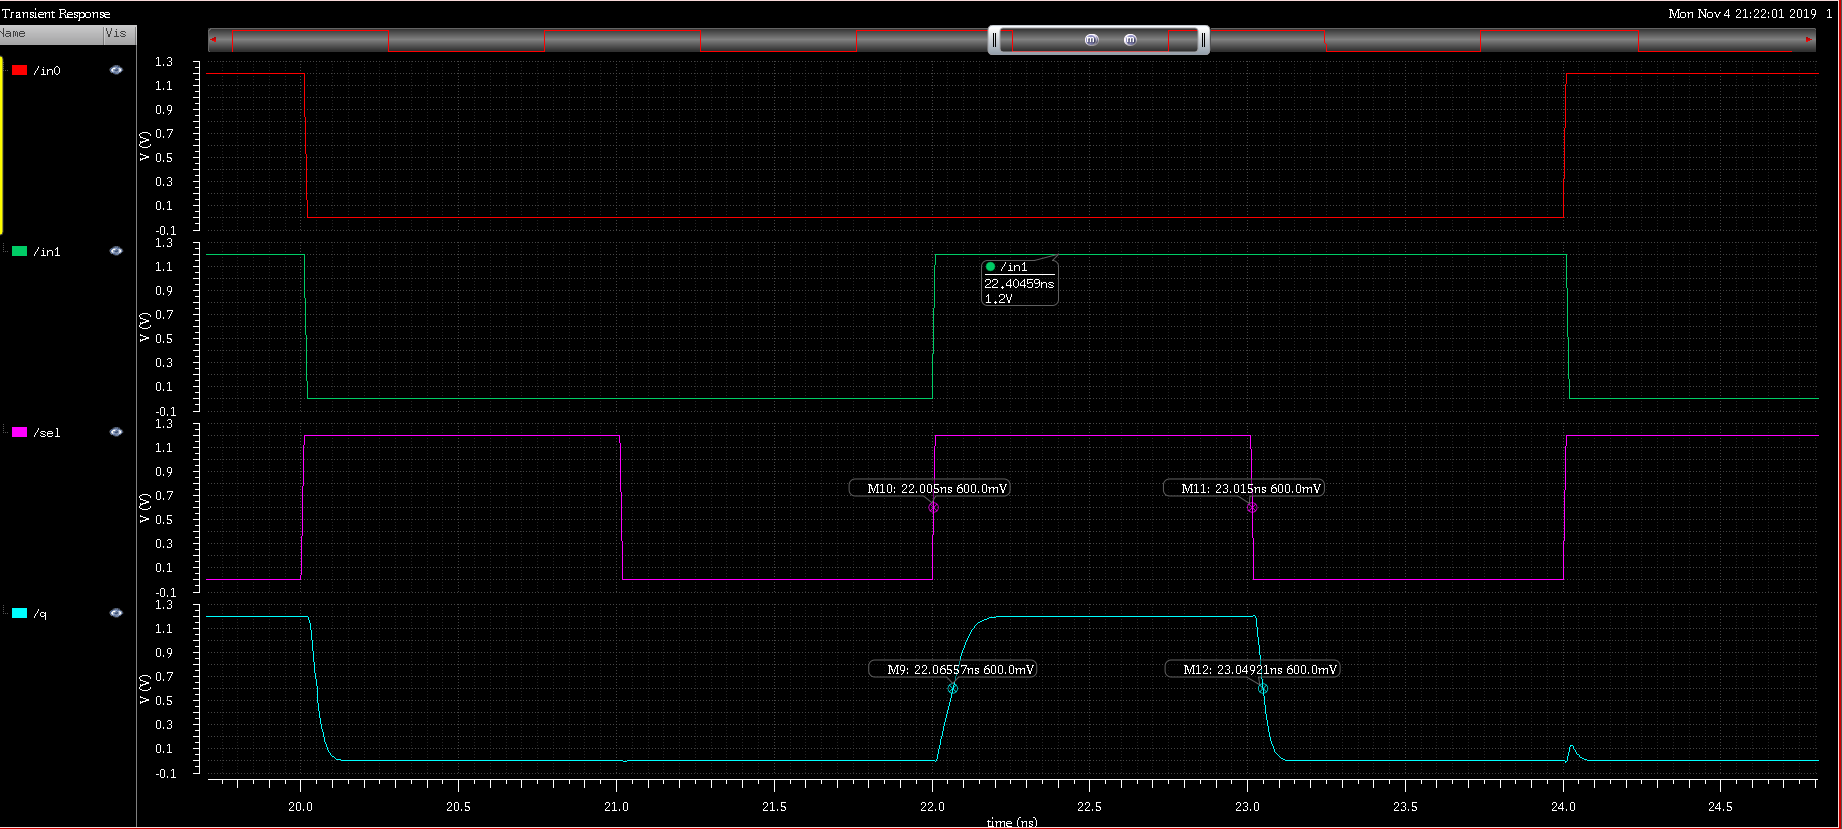
\includegraphics[width=\textwidth]{mux_prop_delay_2.png}
		\caption{Second configuration's propagation delays}
		\label{fig5b}
	\end{subfigure}
	\caption{Output propagation delays with respect to SEL input signal}
\end{figure}


It is clear that the propagation rising and falling delays of the 2 cases are not equal. Hence, the worst-case propagation delay is the average of the worst-case rising propagation delay and the worst-case falling propagation delay. According to table \ref{table2}, $t_{pdr worst} = 0.06057$, $t_{pdf worst} = 0.04496$, and $t_{pd} = \frac{0.06057+0.04496}{2} = 0.052765$.

In addition, the rise time and fall time of the mux can also be extracted from the simulation in Figure \ref{fig6a} \& \ref{fig6b}.

\begin{figure}[htb!]
	\centering
	\begin{subfigure}[htb]{.9\linewidth}
		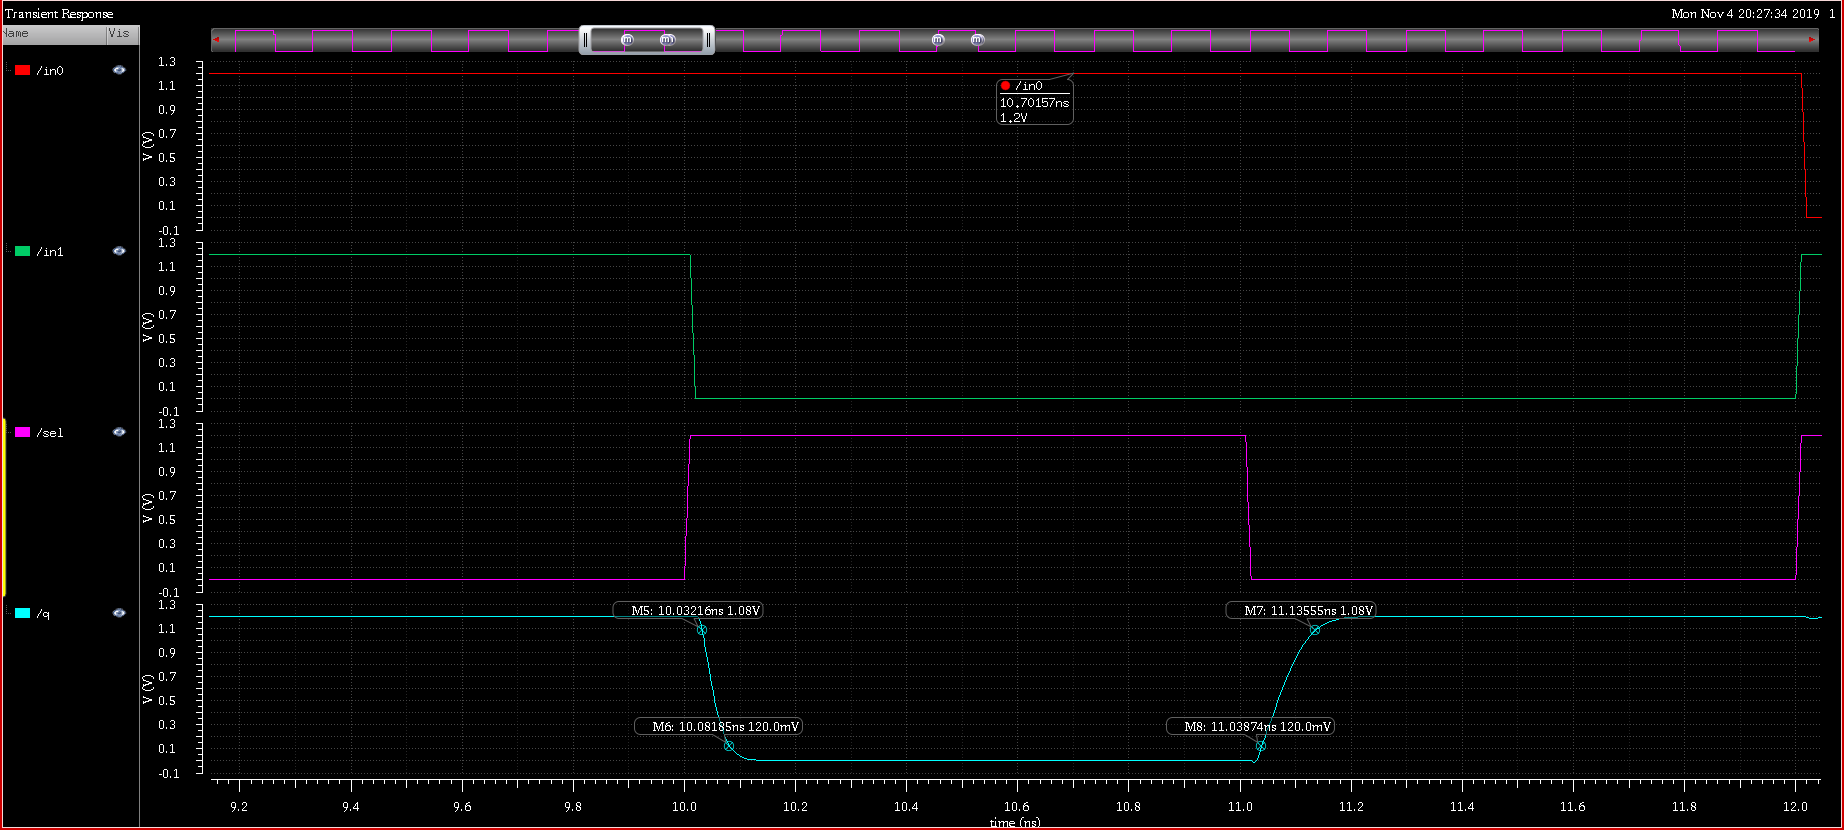
\includegraphics[width=\textwidth]{mux_rise_fall_time_1.png}
		\caption{First configuration's rising and falling time}
		\label{fig6a}
	\end{subfigure}
	%	\hskip2em
	\begin{subfigure}[htb]{.9\linewidth}
		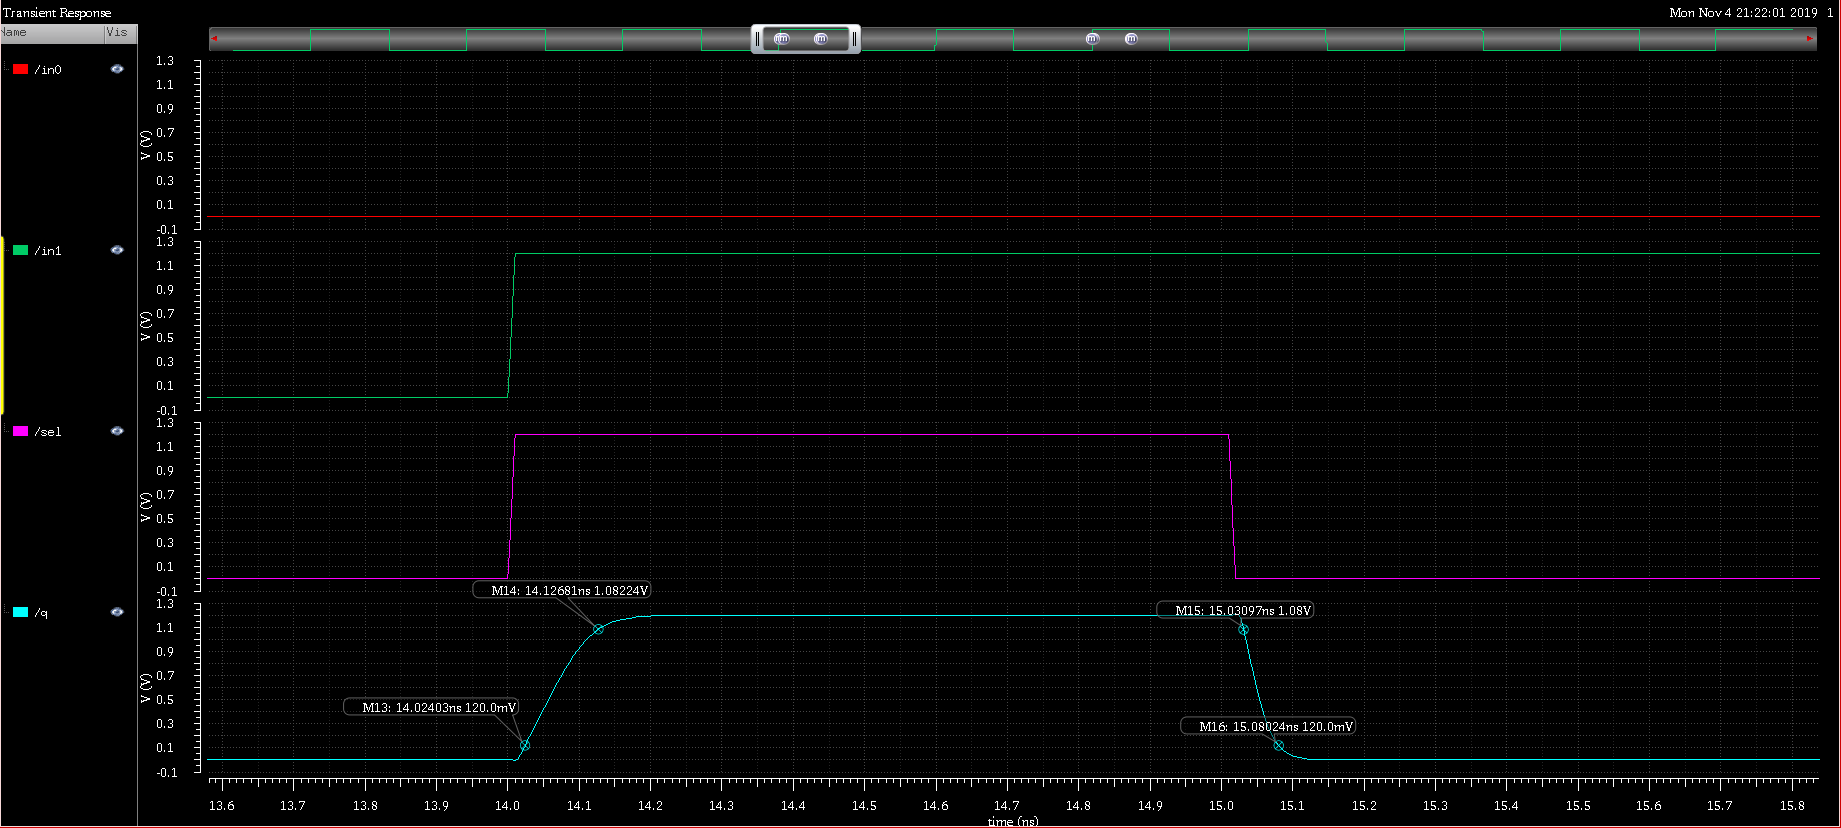
\includegraphics[width=\textwidth]{mux_rise_fall_time_2.png}
		\caption{Second configuration's rising and falling time}
		\label{fig6b}
	\end{subfigure}
	\caption{Rising and falling output time of the 2-to-1 mux}
\end{figure}

\pagebreak
From the 2 figures above, it can be concluded that the worst-case rising time is 0.10278 ($>0.0968$), which results from configuration 2 and the worst-case falling time is 0.0497 ($>0.0493$), which results from configuration 1.


\pagebreak
\section{Layout Design and Verification Results}
\label{sec:layout_desg_and_verification}

This section features the layout design (Figure \ref{fig7}) of the 2-to-1 mux and its verification results, done in the Virtuoso Layout Suite. The design shown below follows strictly the logic gate schematic connections in Figure \ref{fig2}. In addition, all inputs and output pins are connected to a higher metal layer, which is a good design consideration because the resulting mux layout will be easier to integrate into larger circuit.

\begin{figure}[htb!]
	\centering
	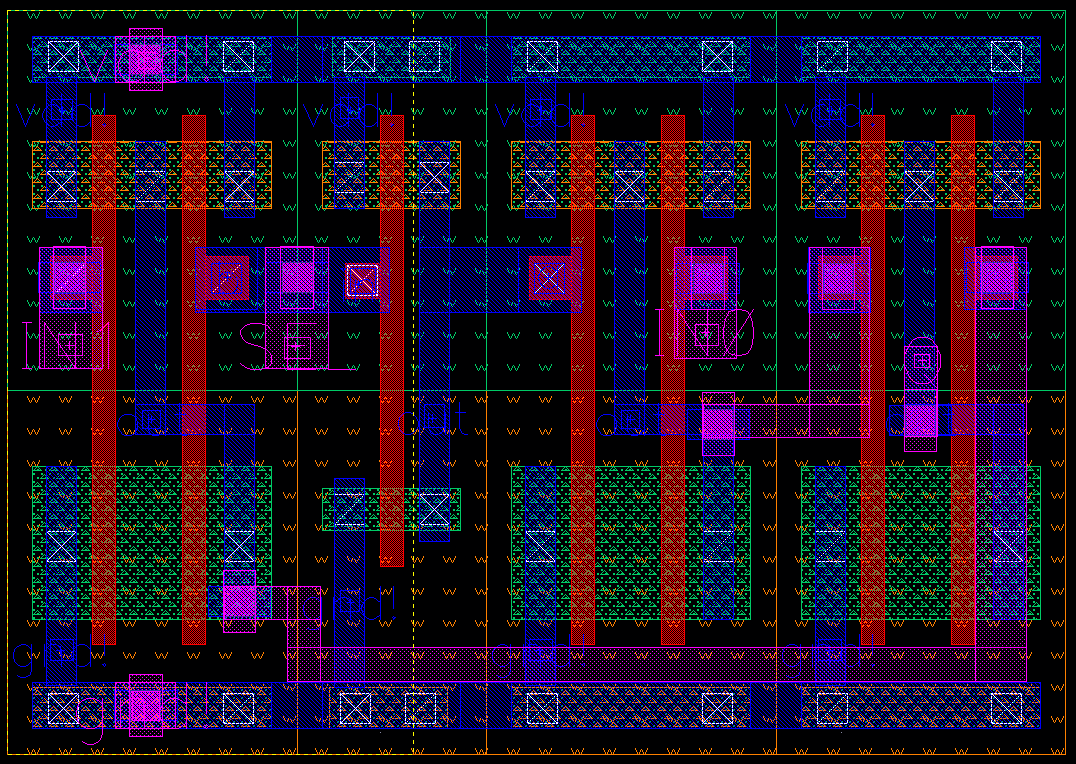
\includegraphics[width=1\linewidth]{mux_layout_final.png}
	\caption{2-to-1 mux layout in Virtuoso Layout Suite}
	\label{fig7}
\end{figure}
\newpage
With this design layout, the DRC and LVS physical verification results are shown below (Figure \ref{fig8a} \& \ref{fig8b}).

\begin{figure}[htb!]
	\centering
	\begin{subfigure}[htb]{.9\linewidth}
		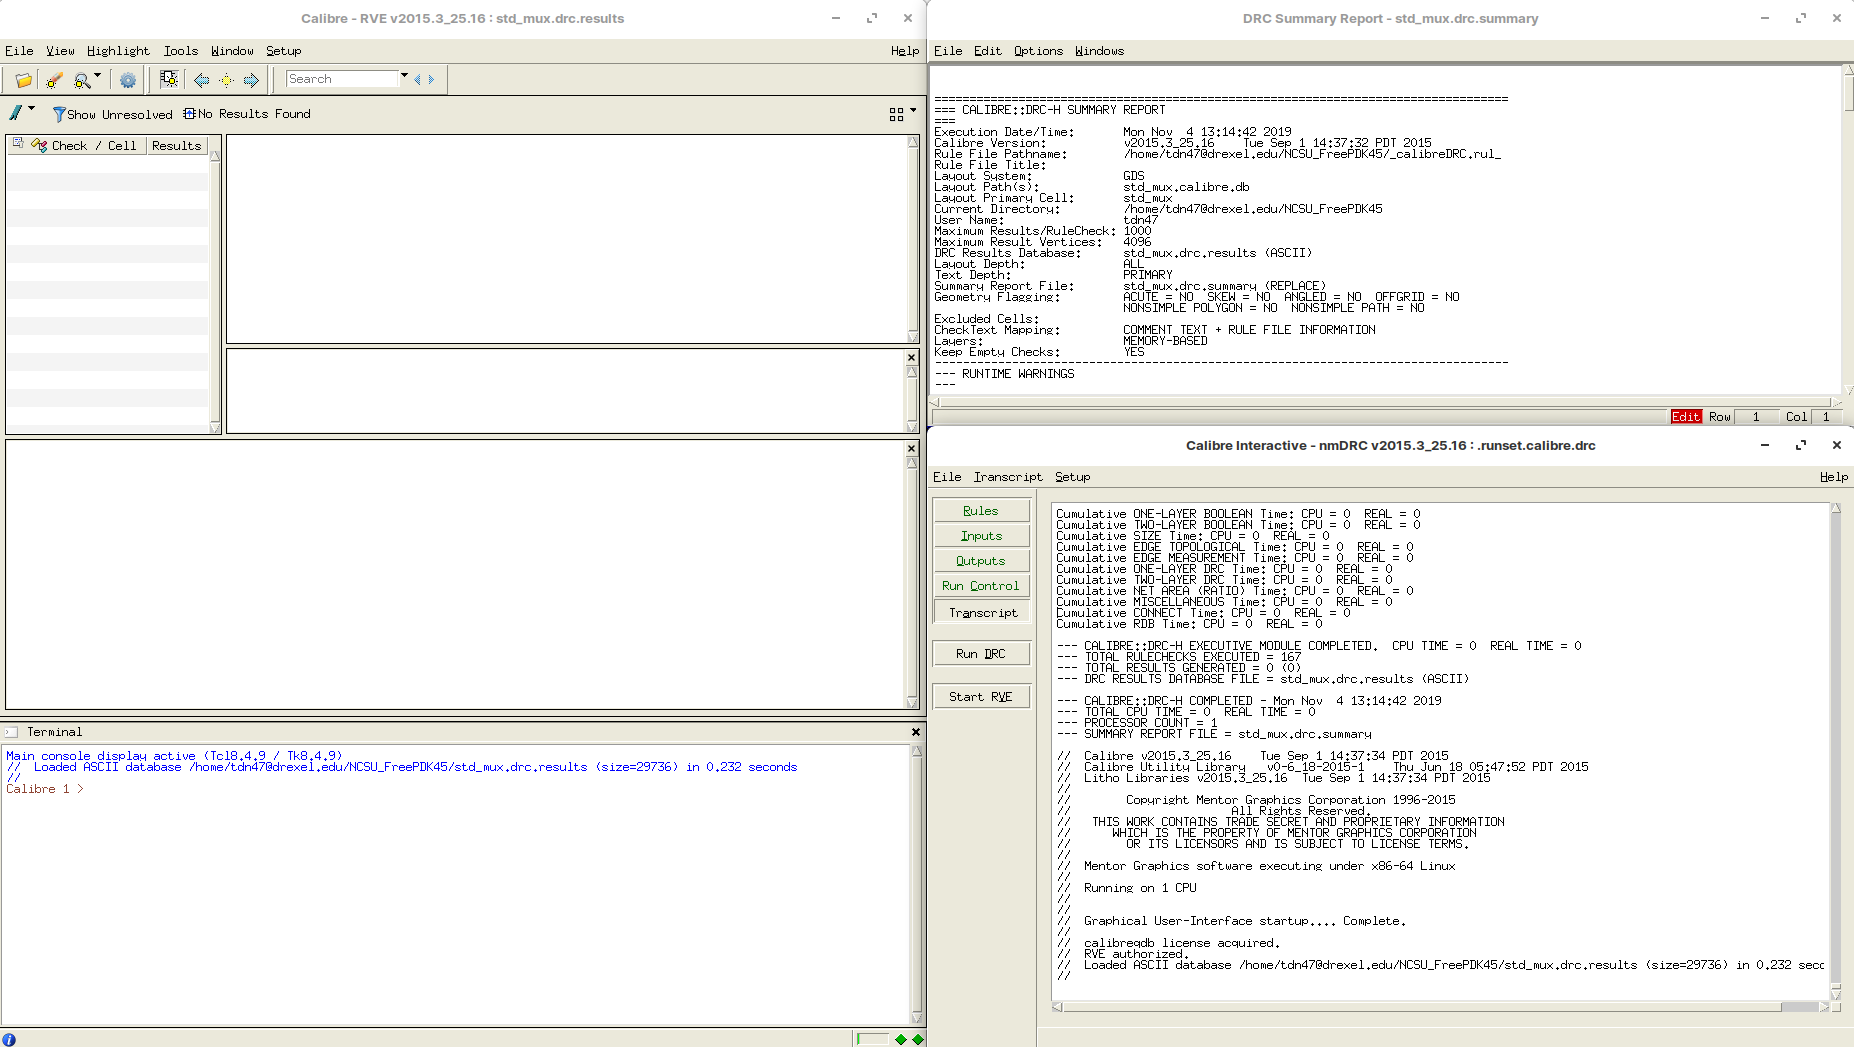
\includegraphics[width=\textwidth]{mux_drc_final.png}
		\caption{DRC Verification Results}
		\label{fig8a}
	\end{subfigure}
	%	\hskip2em
	\begin{subfigure}[htb]{.9\linewidth}
		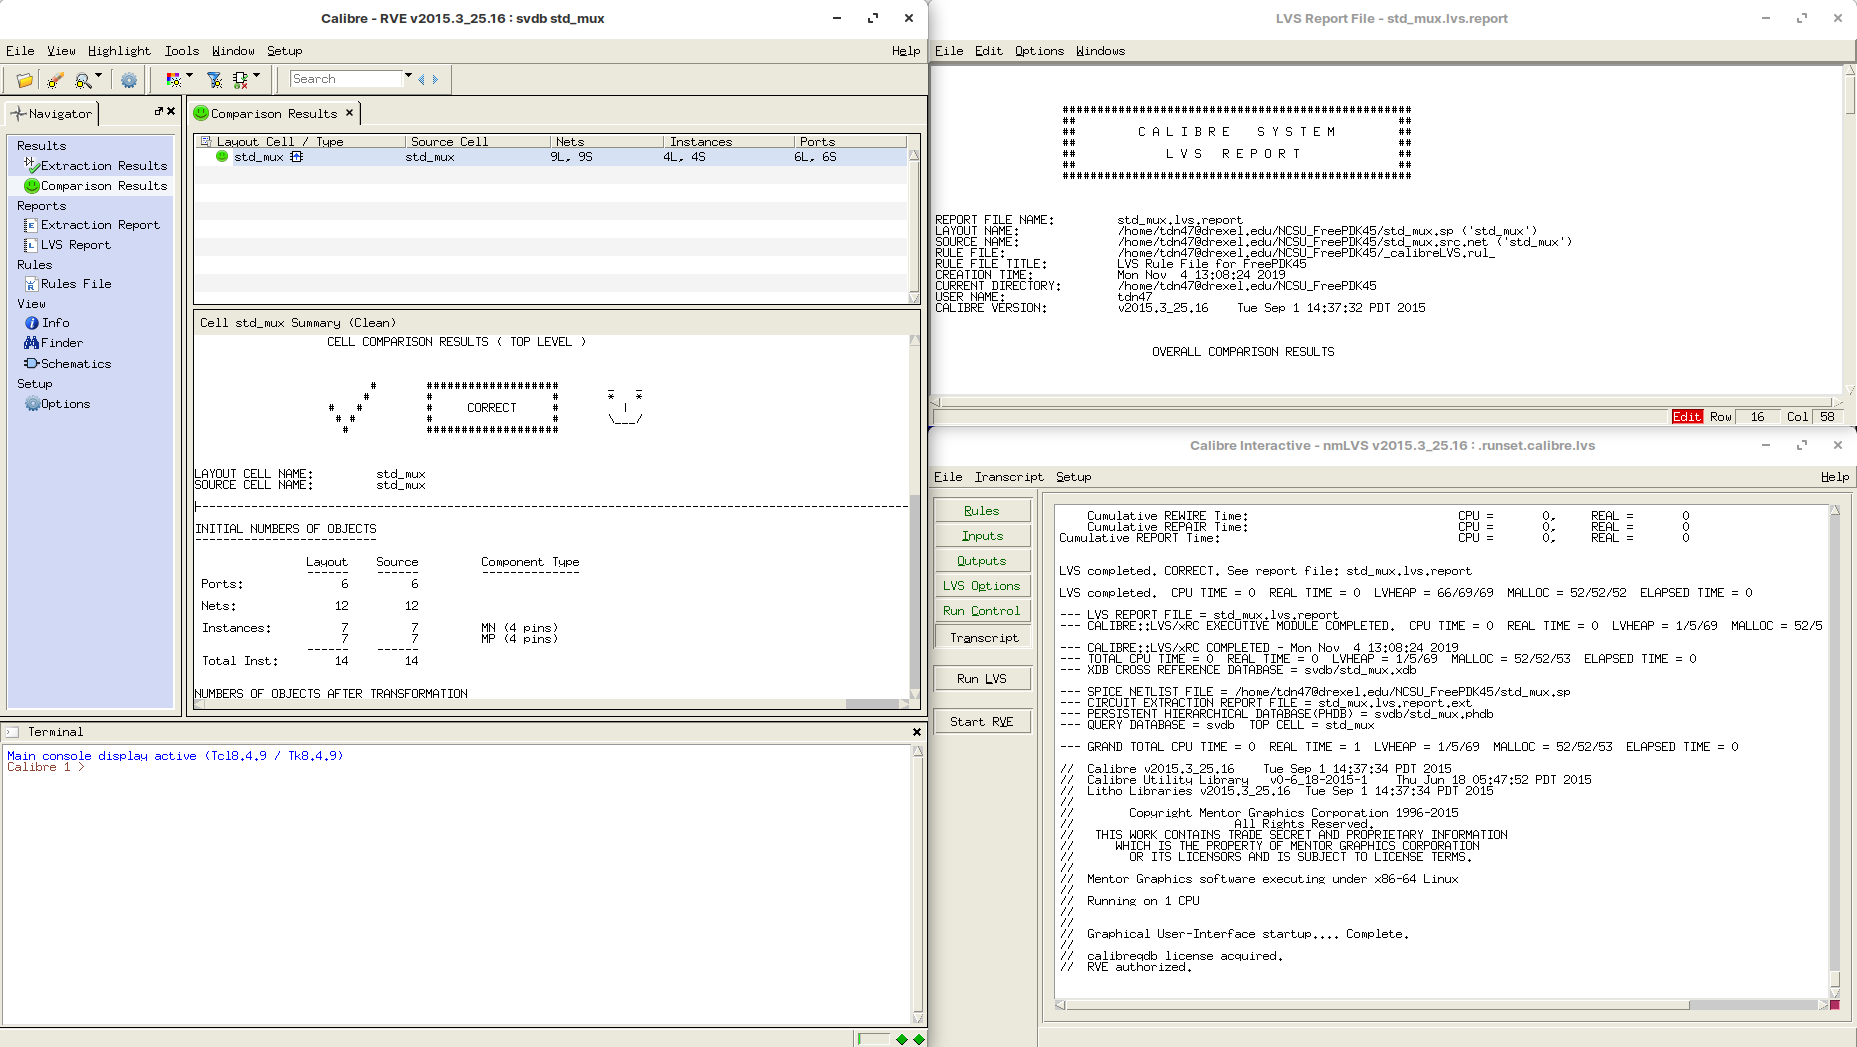
\includegraphics[width=\textwidth]{mux_lvs_final.png}
		\caption{LVS Verification Results}
		\label{fig8b}
	\end{subfigure}
	\caption{2-to-1 mux layout's verification results}
\end{figure}
\newpage

\section{Discussion and Conclusion}
\label{sec:disc_and_concl}

This laboratory explores the design and characteristic of such design for a 2-to-1 multiplexer. From the simulation results above, the mux's rising propagation delay is generally higher than its falling propagation delay. This phenomenon is due to the fact that when the output is 1, one of the two NAND gates has to be 1, which means that the network is trying to charge 4 PMOS, resulting in higher delay. When the output is 0, both input NAND gates have to be 1, hence either path will only result in charging 2 PMOS. According to Table \ref{table2}, the combination (IN0=0, IN1=1, SEL=1, Q=1) means that the output NAND is on, the upper input NAND is on and the inverter is on, which results in the network having to charge the PMOSes of 2 NAND gates and going through an inverter (whose PMOS capacitance does contribute to the output capacitance). Hence, that combination gives the highest delay. The reasoning for the resulting numbers from the other 3 cases follow the same pattern.


\end{document}